\documentclass[12pt]{article}

% Core math
\usepackage{amsmath, amssymb, amsthm}

% Diagrams
\usepackage{tikz-cd}
\usepackage{tikz}

% References
\usepackage{hyperref}
\usepackage{cleveref}

% Graphics
\usepackage{graphicx}

% Page layout
\usepackage[margin=1in]{geometry}

% GrokRxiv sidebar
\usepackage{everypage}
\usepackage{xcolor}

% Code listings
\usepackage{listings}

% Enumerate options (label=(\roman*), etc.)
\usepackage{enumitem}

% Theorem environments
\newtheorem{theorem}{Theorem}[section]
\newtheorem{proposition}[theorem]{Proposition}
\newtheorem{lemma}[theorem]{Lemma}
\newtheorem{corollary}[theorem]{Corollary}
\theoremstyle{definition}
\newtheorem{definition}[theorem]{Definition}
\newtheorem{example}[theorem]{Example}
\theoremstyle{remark}
\newtheorem{remark}[theorem]{Remark}

% GrokRxiv sidebar
\definecolor{grokgray}{RGB}{110,110,110}
\AddEverypageHook{%
  \ifnum\value{page}=1
    \begin{tikzpicture}[remember picture, overlay]
      \node[
        rotate=90,
        anchor=south,
        font=\Large\sffamily\bfseries\color{grokgray},
        inner sep=0pt
      ] at ([xshift=38pt, yshift=0.52\paperheight]current page.south west)
      {GrokRxiv:2026.05.set-theoretic-perspective\quad
       [\,math.LO\,]\quad
       03 May 2026};
    \end{tikzpicture}
  \fi
}

% Listings setup for Haskell
\lstdefinelanguage{Haskell}{
  morekeywords={data, where, let, in, do, case, of, if, then, else, type, newtype, class, instance, module, import, deriving},
  sensitive=true,
  morecomment=[l]{--},
  morecomment=[s]{\{-}{-\}},
  morestring=[b]"
}
\lstset{
  basicstyle=\ttfamily\small,
  keywordstyle=\color{blue!70!black}\bfseries,
  commentstyle=\color{green!50!black}\itshape,
  stringstyle=\color{red!70!black},
  showstringspaces=false,
  breaklines=true,
  frame=single,
  framesep=4pt,
  language=Haskell
}

\title{The Set-Theoretic Perspective: \\
Numbers as von Neumann Ordinals \\
\large Paper 02 of the Univalent Correspondence Series}

\author{YonedaAI Research \\
\textit{Formalized Foundations of Mathematics Project} \\
\textit{Univalent Correspondence Series} \\
\texttt{research@yonedaai.com}}

\date{03 May 2026}

\begin{document}

\maketitle

\begin{abstract}
We examine the second of six perspectives in the Univalent Correspondence series:
the set-theoretic level, in which natural numbers are reduced to particular
elements of the cumulative hierarchy of pure sets. We work primarily in
Zermelo--Fraenkel set theory with Choice (ZFC), focusing on John von Neumann's
ordinal encoding $0 = \emptyset$, $n+1 = n \cup \{n\}$, where the natural number
$58$ is realized as the set $\{0,1,\ldots,57\}$ of all smaller von Neumann
ordinals. We contrast this with Ernst Zermelo's earlier encoding
$0 = \emptyset$, $n+1 = \{n\}$, in which $58$ is realized as a chain of $58$
nested singletons. Both encodings produce structures isomorphic to
$(\mathbb{N},0,\mathrm{succ})$ as Peano models, yet they differ on
\emph{internal} set-theoretic questions such as whether $2 \in 3$ or whether
$\{\emptyset\} \in 17$. Following Paul Benacerraf's 1965 paper
\emph{What Numbers Could Not Be}, we argue that this discrepancy is not a
defect to be eliminated but a structural fact: numbers are not sets, and any
attempt to identify them with sets generates encoding-relative
\emph{junk theorems} that are meaningful about the encoding but meaningless
about the number. We give a careful presentation of the ZFC axiomatization,
the cumulative hierarchy $V_\alpha$, ranks, and well-foundedness; we define
addition, multiplication, and order recursively on the von Neumann ordinals
and verify that these definitions satisfy the Peano axioms; and we prove a
general representation theorem stating that any successor structure obtained
from a class function $S$ that is injective, has a base point not in its
image, and admits transfinite iteration generates a model of Peano arithmetic
isomorphic to the von Neumann naturals. We close with a structuralist
re-reading: the set-theoretic perspective \emph{does} present numbers, but
only as encodings; the structural content these encodings share is a
universal property, which Paper 03 will make explicit. Our development is
accompanied by a Haskell implementation that realizes both encodings as
distinct types and proves, by construction, that they satisfy the same Peano
interface.
\end{abstract}

\tableofcontents

\newpage

\section{Introduction}
\label{sec:intro}

\subsection{Where we are in the series}

This is the second paper in a six-paper series, plus a synthesis volume,
exploring the question \emph{``what is a natural number?''} at progressively
higher levels of mathematical abstraction. Paper 01 considered the
\emph{naive} level, in which a number is treated as a primitive symbol or
quantity, without further analysis. The naive level is the practical
starting point of arithmetic and the inevitable surface of any numeral
system, but it conflates syntax with semantics: the symbols ``$58$'',
``LVIII'', and ``$\underbrace{\vert\vert\cdots\vert}_{58}$'' all refer to
the same number, but the naive level provides no machinery for distinguishing
the numeral from the number it names.

The natural next step, taken in the foundational programs of the early
twentieth century, is to \emph{reduce} numbers to objects of a more basic
theory. Frege \cite{frege1884} attempted such a reduction to logic; Russell
and Whitehead refined and elaborated it in \emph{Principia Mathematica}
\cite{principia}; Zermelo and later Fraenkel and Skolem developed the
axiomatic set theory we now call ZFC. Within ZFC, John von Neumann
\cite{vonNeumann1923} gave a canonical recursive definition of the ordinals
that, when restricted to the finite case, produces a particular set-theoretic
implementation of the natural numbers. Standard expositions of the resulting
machinery include Halmos \cite{halmos1960}, Suppes \cite{suppes1960},
Shoenfield \cite{shoenfield1967}, and Kunen \cite{kunen1980}.

\subsection{The thesis of this paper}

We make four claims:

\begin{enumerate}
\item \textbf{Set theory does provide a foundation for arithmetic.} The von
Neumann encoding inside ZFC produces a structure
$(\omega, 0, \mathrm{succ})$, where $\omega$ is the smallest inductive set, on
which addition, multiplication, and order can be defined recursively, and
which satisfies the (second-order) Peano axioms.

\item \textbf{The encoding is not unique.} Zermelo's earlier encoding,
$0 = \emptyset$, $n+1 = \{n\}$, gives a different set-theoretic structure
that nevertheless also satisfies the Peano axioms. Many other encodings exist.
The encodings are mutually \emph{Peano-isomorphic} but not mutually
\emph{ZFC-isomorphic}: as sets, they differ.

\item \textbf{The discrepancy generates junk theorems.} In von Neumann's
encoding, $2 \in 3$ is true; in Zermelo's, it is false. The question
``is $2$ an element of $3$?'' is meaningful inside ZFC for each
encoding separately, but it is meaningless about \emph{the number} $2$ ---
it is an artifact of the encoding. Following Benacerraf \cite{benacerraf1965},
we conclude that numbers cannot be identified with sets.

\item \textbf{The structural content survives.} What both encodings share
is precisely the universal property of a Natural Number Object: they are both
initial in a category of pointed sets with endomorphism. This is the
structural content that Paper 03 will make explicit. The set-theoretic
perspective is therefore not refuted but \emph{relocated}: it is one
implementation of a structural specification, not a definition.
\end{enumerate}

\subsection{Outline}

\Cref{sec:zfc} reviews ZFC, with particular attention to the axiom of
infinity, the axiom schema of replacement, and the foundation axiom (which
underwrites well-foundedness). \Cref{sec:vN} presents the von Neumann
encoding, defines $\omega$, and verifies the Peano axioms. \Cref{sec:zermelo}
presents Zermelo's encoding and contrasts the two. \Cref{sec:benacerraf}
develops Benacerraf's identification problem and the notion of a junk
theorem. \Cref{sec:operations} defines addition, multiplication, and order
recursively and proves the basic algebraic identities. \Cref{sec:cumulative}
introduces the cumulative hierarchy $V_\alpha$, ranks, and well-foundedness,
and locates the natural numbers within it. \Cref{sec:representation} proves
a representation theorem characterizing successor structures up to
isomorphism. \Cref{sec:bridge} develops the structuralist re-reading and
sketches the bridge to Paper 03. The Haskell implementation accompanying the
paper realizes both encodings; \Cref{sec:haskell} describes its design and
the Peano-axiom verification by construction.

\section{Mathematical Framework: ZFC Reviewed}
\label{sec:zfc}

We work in classical first-order logic with equality and a single binary
relation symbol $\in$.

\subsection{Axioms}

\begin{definition}[ZFC]\label{def:zfc}
The axioms of Zermelo--Fraenkel set theory with Choice are:

\begin{enumerate}
\item[\textbf{(Ext)}] \emph{Extensionality.}
$\forall x\, \forall y\, \bigl(\forall z\,(z \in x \leftrightarrow z \in y) \to x = y\bigr)$.

\item[\textbf{(Pair)}] \emph{Pairing.}
$\forall x\, \forall y\, \exists z\, \forall w\,(w \in z \leftrightarrow w = x \vee w = y)$.

\item[\textbf{(Un)}] \emph{Union.}
$\forall x\, \exists y\, \forall z\,(z \in y \leftrightarrow \exists w\,(w \in x \wedge z \in w))$.

\item[\textbf{(Pow)}] \emph{Power set.}
$\forall x\, \exists y\, \forall z\,(z \in y \leftrightarrow z \subseteq x)$.

\item[\textbf{(Sep)}] \emph{Separation schema.} For each formula $\varphi(z)$
not involving $y$,
$\forall x\, \exists y\, \forall z\,(z \in y \leftrightarrow z \in x \wedge \varphi(z))$.

\item[\textbf{(Repl)}] \emph{Replacement schema.} For each formula
$\varphi(x,y)$ defining a class function $F$,
\[
\forall A\, \exists B\, \forall y\,
   \bigl(y \in B \leftrightarrow \exists x \in A\,\, \varphi(x,y)\bigr).
\]

\item[\textbf{(Inf)}] \emph{Infinity.}
$\exists I\,\bigl(\emptyset \in I \wedge \forall x\,(x \in I \to x \cup \{x\} \in I)\bigr)$.

\item[\textbf{(Found)}] \emph{Foundation.}
$\forall x\,(x \neq \emptyset \to \exists y \in x\,(y \cap x = \emptyset))$.

\item[\textbf{(AC)}] \emph{Choice.} Every set of nonempty sets has a choice
function.
\end{enumerate}
\end{definition}

\begin{remark}
The empty set $\emptyset$ is definable: by Separation applied to any set $x$
and the formula $z \neq z$, the resulting set has no elements. By Extensionality,
this set is unique. \textbf{(Inf)} guarantees there is a set containing $\emptyset$
and closed under $x \mapsto x \cup \{x\}$.
\end{remark}

\subsection{Axiom of Infinity, in detail}

\begin{definition}[Inductive set]
A set $I$ is \emph{inductive} when $\emptyset \in I$ and, for every $x \in I$,
$x \cup \{x\} \in I$. The axiom of infinity asserts that an inductive set exists.
\end{definition}

\begin{proposition}[Existence of $\omega$]\label{prop:omega}
There exists a unique smallest inductive set, denoted $\omega$. Equivalently,
$\omega = \bigcap \{I : I \text{ is inductive}\}$ inside any inductive set,
defined by Separation:
\begin{equation}
\omega = \{x \in I_0 : \forall I\,(I \text{ inductive} \to x \in I)\},
\end{equation}
where $I_0$ is any fixed inductive set guaranteed by \textbf{(Inf)}.
\end{proposition}

\begin{proof}
The class of inductive sets is nonempty by \textbf{(Inf)}; the
class-intersection is inductive (it contains $\emptyset$ since each inductive
set does, and is closed under $x \mapsto x \cup \{x\}$ since each inductive
set is). Separation applied to $I_0$ and the formula
$\varphi(x) \equiv \forall I\,(\text{Ind}(I) \to x \in I)$ produces a set $\omega$
with the required property. Uniqueness follows from Extensionality.
\end{proof}

\subsection{Replacement, and what it buys us}

The Separation schema only carves out subsets of an existing set; it cannot
generate sets ``larger'' than what is already given. Replacement is strictly
stronger: it asserts that the image of a set under a definable class function
is a set. This is essential for transfinite recursion (and hence for the
cumulative hierarchy of \Cref{sec:cumulative}) and for the formal definition
of operations such as addition by recursion on $\omega$.

\begin{remark}
ZFC without Replacement is Zermelo's original 1908 system $\mathrm{Z}$, which
is too weak for many constructions used in ordinary mathematics (Borel
hierarchies, transfinite recursion past $\omega + \omega$, etc.). For our
purposes here --- defining the natural numbers and their arithmetic ---
Replacement is the crucial axiom that lets us define functions by recursion.
\end{remark}

\subsection{Foundation and well-foundedness}

\begin{definition}[Well-founded relation]
A relation $R$ on a class $C$ is \emph{well-founded} when every nonempty
subset $S \subseteq C$ has an $R$-minimal element: an $x \in S$ with
$\{y \in S : yRx\} = \emptyset$.
\end{definition}

\begin{theorem}\label{thm:found}
The Foundation axiom is equivalent (in ZF without Foundation) to the
assertion that the membership relation $\in$ is well-founded on the universe
of sets. In particular, there is no infinite descending $\in$-chain
$\cdots \in x_2 \in x_1 \in x_0$, no set $x$ with $x \in x$, and no cycle
$x_0 \in x_1 \in \cdots \in x_n \in x_0$.
\end{theorem}

\begin{proof}[Proof sketch]
If $x \in x$, then $\{x\}$ has no $\in$-minimal element, contradicting
Foundation. The general statement is proved by considering the transitive
closure of any candidate descending chain and applying Foundation to the
resulting set.
\end{proof}

Foundation is what allows transfinite induction on the entire set-theoretic
universe. It is also what makes the von Neumann encoding (in which $n$ is
literally the set of its predecessors) compatible with the standard
machinery: since each $n$ is a transitive set linearly ordered by $\in$,
Foundation guarantees we never run into pathologies like $n \in n$.

\section{The von Neumann Encoding}
\label{sec:vN}

\subsection{Definition}

\begin{definition}[Successor]\label{def:succ}
For any set $x$, the \emph{successor} of $x$ is
$x^+ := x \cup \{x\}$.
\end{definition}

\begin{definition}[Von Neumann naturals]\label{def:vN}
We define the von Neumann naturals as elements of $\omega$ recursively:
\begin{align}
0_{\mathrm{vN}} &:= \emptyset, \\
(n+1)_{\mathrm{vN}} &:= (n_{\mathrm{vN}})^+ = n_{\mathrm{vN}} \cup \{n_{\mathrm{vN}}\}.
\end{align}
\end{definition}

Unrolling this definition:
\begin{align*}
0 &= \emptyset \\
1 &= \{0\} = \{\emptyset\} \\
2 &= \{0, 1\} = \{\emptyset, \{\emptyset\}\} \\
3 &= \{0, 1, 2\} = \{\emptyset, \{\emptyset\}, \{\emptyset, \{\emptyset\}\}\} \\
&\vdots \\
n &= \{0, 1, \ldots, n-1\}
\end{align*}

\begin{example}\label{ex:58}
The number $58$, in von Neumann form, is the set of all smaller naturals:
\begin{equation}
58_{\mathrm{vN}} = \{0, 1, 2, \ldots, 57\}.
\end{equation}
The set $58$ has exactly $58$ elements, and each of those elements is a set
with strictly fewer elements. The total cumulative count of $\in$-occurrences
inside $58$ is large but finite (combinatorially, $\sum_{k=0}^{57} k = 1653$).
\end{example}

\subsection{Membership and subset coincide}

A signal feature of the von Neumann encoding is the conflation, at the
finite level, of $\in$ and $\subseteq$.

\begin{proposition}\label{prop:in-equals-subset}
For all $m, n \in \omega$, we have $m \in n$ if and only if $m \subsetneq n$.
\end{proposition}

\begin{proof}
We prove both directions by induction on $n$.

\emph{$(\Rightarrow)$.} If $m \in n$, then since $n$ is the set of its
predecessors and is transitive (\Cref{prop:transitive} below), every element
of $m$ is also an element of $n$, hence $m \subseteq n$. Strict inclusion
follows from $m \in n$ and $m \notin m$ (Foundation, \Cref{thm:found}).

\emph{$(\Leftarrow)$.} If $m \subsetneq n$, pick any $k \in n \setminus m$
of minimal $\in$-rank. Then $k \subseteq m$ (by minimality), and $k = m$
follows from extensionality together with $m \subseteq n$ and the definition
of $n$ as the set of its predecessors. Hence $m = k \in n$.
\end{proof}

\begin{proposition}[Transitivity of naturals]\label{prop:transitive}
Each $n \in \omega$ is a \emph{transitive set}: if $x \in n$, then $x \subseteq n$.
\end{proposition}

\begin{proof}
By induction. $0 = \emptyset$ is vacuously transitive. Assume $n$ is
transitive and let $x \in n^+ = n \cup \{n\}$. If $x = n$, then $x = n \subseteq n^+$
since $n \cup \{n\} \supseteq n$. If $x \in n$, then by the inductive
hypothesis $x \subseteq n \subseteq n^+$.
\end{proof}

\begin{example}
$2 \in 3$ holds in von Neumann: $3 = \{0,1,2\}$, so $2$ is literally one of the
three elements of $3$. Equivalently, $2 = \{0,1\} \subsetneq \{0,1,2\} = 3$.
This is the kind of statement that, by \Cref{prop:in-equals-subset}, is
equivalent in von Neumann to the order $2 < 3$.
\end{example}

\subsection{Peano axioms for the von Neumann naturals}

\begin{theorem}\label{thm:peano-vN}
The structure $(\omega, 0_{\mathrm{vN}}, (\cdot)^+)$ satisfies the Peano axioms:
\begin{enumerate}
\item $0_{\mathrm{vN}} \in \omega$.
\item For all $n \in \omega$, $n^+ \in \omega$.
\item For all $n \in \omega$, $n^+ \neq 0_{\mathrm{vN}}$.
\item For all $m,n \in \omega$, if $m^+ = n^+$ then $m = n$.
\item (Induction) For every set $S \subseteq \omega$, if $0_{\mathrm{vN}} \in S$
and $S$ is closed under $(\cdot)^+$, then $S = \omega$.
\end{enumerate}
\end{theorem}

\begin{proof}
\textbf{(1) and (2)} are immediate from the definition of $\omega$ as the
smallest inductive set.

\textbf{(3)} If $n^+ = \emptyset$, then $n \cup \{n\} = \emptyset$. But
$n \in n \cup \{n\}$, contradiction.

\textbf{(4)} Suppose $m^+ = n^+$, i.e.\ $m \cup \{m\} = n \cup \{n\}$. Then
$m \in n^+$ and $n \in m^+$. By \Cref{prop:in-equals-subset} (applied via
$\in$-trichotomy), if $m \neq n$ then either $m \in n$ and $n \in m$, which
contradicts Foundation, or one is a proper subset of the other; combined
with $m \in n^+$ and $n \in m^+$ this forces $m = n$.

\textbf{(5)} Let $S \subseteq \omega$ be inductive (containing $0$ and
closed under $(\cdot)^+$). Then $S$ itself is an inductive set, so
$\omega \subseteq S$ by minimality of $\omega$. The reverse inclusion is by
hypothesis.
\end{proof}

\section{Zermelo's Encoding}
\label{sec:zermelo}

Ernst Zermelo, in his 1908 axiomatization \cite{zermelo1908}, used a
different recursive definition of the natural numbers.

\begin{definition}[Zermelo naturals]\label{def:Z}
We define the Zermelo naturals recursively:
\begin{align}
0_{\mathrm{Z}} &:= \emptyset, \\
(n+1)_{\mathrm{Z}} &:= \{n_{\mathrm{Z}}\}.
\end{align}
\end{definition}

Unrolling:
\begin{align*}
0_{\mathrm{Z}} &= \emptyset \\
1_{\mathrm{Z}} &= \{\emptyset\} \\
2_{\mathrm{Z}} &= \{\{\emptyset\}\} \\
3_{\mathrm{Z}} &= \{\{\{\emptyset\}\}\} \\
&\vdots \\
n_{\mathrm{Z}} &= \underbrace{\{\{\cdots\{}_{n}\emptyset\underbrace{\}\cdots\}\}}_{n}
\end{align*}

\begin{example}
$58_{\mathrm{Z}}$ is a chain of $58$ nested singletons:
\begin{equation}
58_{\mathrm{Z}} = \underbrace{\{\{\cdots\{}_{58}\emptyset\underbrace{\}\cdots\}\}}_{58}.
\end{equation}
Crucially, $58_{\mathrm{Z}}$ has exactly \emph{one} element (namely
$57_{\mathrm{Z}}$), not $58$. The cardinality of the encoding does not match
the natural number it encodes.
\end{example}

\subsection{Comparison: junk theorems}

\begin{proposition}[Encoding-relative facts]\label{prop:junk}
The following statements all have determinate truth values inside ZFC, but
the answers depend on the encoding. We display together the cases where the
encodings agree and where they differ. (Below, $\mathrm{pred}(n)$ denotes
the ordinal predecessor: the unique $m$ with $m^+ = n$.)
\begin{center}
\begin{tabular}{lll}
\textbf{Question} & \textbf{Von Neumann} & \textbf{Zermelo} \\\hline
$0 \in 1$? & true & true (both: $1 = \{0\}$) \\
$n \in n^+$? & true & true (by construction) \\
$n \subseteq n^+$? & true & true \\
$1 \in 3$? & true ($3 = \{0,1,2\}$) & \textbf{false} ($3_{\mathrm{Z}} = \{2_{\mathrm{Z}}\}$) \\
$1 \in 17$? & true & \textbf{false} \\
$\{\emptyset\} \in 17$? & true (since $\{\emptyset\} = 1 \in 17$) & \textbf{false} \\
$|n| = n$ for $n \in \omega$? & true (each $n$ has $n$ elements) & \textbf{false} ($|n|=1$ for $n \geq 1$) \\
$\bigcup n = \mathrm{pred}(n)$ for $n>0$? & true & true \\
$m \subsetneq n \iff m \in n$ (on $\omega$)? & true & \textbf{false}
\end{tabular}
\end{center}

Two rows merit closer comment. The cardinality row exhibits the most
striking divergence: $|2_{\mathrm{vN}}| = |\{0,1\}| = 2$ but
$|2_{\mathrm{Z}}| = |\{\{\emptyset\}\}| = 1$, so already at $n=2$ the
extensional ``size'' of the encoding tracks the natural number in von
Neumann but not in Zermelo. For the membership/subset equivalence in the
last row, the von Neumann case holds by \Cref{prop:in-equals-subset}; in
Zermelo it fails. For instance, $1_{\mathrm{Z}} = \{\emptyset\}$ is not a
subset of $2_{\mathrm{Z}} = \{\{\emptyset\}\}$, because the unique element
$\emptyset$ of $1_{\mathrm{Z}}$ is not an element of
$\{\{\emptyset\}\}$. The reliable encoding-independent statement of the
natural order is therefore the structural Peano order $m < n$ (defined,
e.g., as $\exists k > 0.\, m + k = n$), not the literal $\in$ relation.
\end{proposition}

\begin{remark}[On adjacent cases]
For pairs $(m, m+1)$ both encodings agree on $m \in m+1$: in von Neumann
because $m \in m \cup \{m\}$, and in Zermelo because $m \in \{m\}$. The
discrepancy is for non-adjacent pairs $(m, n)$ with $m + 1 < n$, where the
von Neumann encoding has $m \in n$ via transitivity but the Zermelo encoding
has $n_{\mathrm{Z}} = \{(n-1)_{\mathrm{Z}}\}$ as a singleton, so only $n - 1$ is
a member of $n$.
\end{remark}

\begin{proof}[Justification of the table]
Every entry follows directly from the recursive definitions and Foundation.
The pivotal entry for our purposes is the last: in von Neumann, membership
and proper inclusion coincide on $\omega$ (\Cref{prop:in-equals-subset}); in
Zermelo, this fails because (for $n \geq 2$) $n_{\mathrm{Z}}$ has only one
element, while many sets are subsets of it under set-theoretic inclusion.
\end{proof}

\begin{remark}[Junk]
We call statements like ``$2 \in 3$'' \emph{junk theorems} (or
\emph{junk falsehoods}). They have a determinate truth value in ZFC under any
fixed encoding, but they reflect choices made by the encoder, not facts
about the natural numbers as such. The number $2$ does not stand in any
intrinsic membership relation to the number $3$. The membership question is
well-formed only because we have committed to representing numbers as sets;
under a different commitment, the answer changes.
\end{remark}

\subsection{Peano axioms for Zermelo}

\begin{proposition}[Existence of $\omega_{\mathrm{Z}}$]\label{prop:omega-Z}
There exists a unique smallest set $\omega_{\mathrm{Z}}$ containing
$\emptyset$ and closed under the operation $x \mapsto \{x\}$.
\end{proposition}

\begin{proof}
The argument parallels that of \Cref{prop:omega} but uses the alternate
successor. Call a set $J$ \emph{$Z$-inductive} when $\emptyset \in J$ and,
for all $x \in J$, $\{x\} \in J$. By the axiom of infinity \textbf{(Inf)},
the standard inductive set $I_0$ exists; by Pairing, the singleton operation
$x \mapsto \{x\}$ is total. Applying the recursion theorem
(\Cref{thm:recursion} below, whose proof depends only on Replacement
applied to $\omega$ and not on either encoding), the recursion
$f(0) = \emptyset$, $f(n^+) = \{f(n)\}$ defines a function $f: \omega \to V$
whose range is a set $J_0$ by Replacement. The set $J_0$ is $Z$-inductive
by construction. Then by Separation,
\[
\omega_{\mathrm{Z}} := \{x \in J_0 : \forall J\,(\text{$Z$-Ind}(J) \to x \in J)\},
\]
is the smallest $Z$-inductive set; it is unique by Extensionality.
\end{proof}

\begin{theorem}\label{thm:peano-Z}
The structure $(\omega_{\mathrm{Z}}, 0_{\mathrm{Z}}, n \mapsto \{n\})$ satisfies
the Peano axioms.
\end{theorem}

\begin{proof}
\textbf{(1)} $0_{\mathrm{Z}} = \emptyset \in \omega_{\mathrm{Z}}$ by
\Cref{prop:omega-Z}.

\textbf{(2)} If $n \in \omega_{\mathrm{Z}}$, then $\{n\} \in \omega_{\mathrm{Z}}$
by closure of $\omega_{\mathrm{Z}}$ under $x \mapsto \{x\}$.

\textbf{(3)} $\{n\} \neq \emptyset$ since $n \in \{n\}$.

\textbf{(4)} If $\{m\} = \{n\}$, then $m \in \{n\}$, so $m = n$.

\textbf{(5)} Let $S \subseteq \omega_{\mathrm{Z}}$ be $Z$-inductive (containing
$0_{\mathrm{Z}}$ and closed under $x \mapsto \{x\}$). Then $S$ is itself
$Z$-inductive, so $\omega_{\mathrm{Z}} \subseteq S$ by minimality of
$\omega_{\mathrm{Z}}$. The reverse inclusion is by hypothesis.
\end{proof}

\subsection{Iso as Peano models, not as sets}

\begin{theorem}\label{thm:peano-iso}
There is a unique bijection $\Phi: \omega \to \omega_{\mathrm{Z}}$ satisfying
$\Phi(0_{\mathrm{vN}}) = 0_{\mathrm{Z}}$ and
$\Phi(n^+) = \{\Phi(n)\}$ for all $n$. The bijection $\Phi$ is an isomorphism
of Peano structures.
\end{theorem}

\begin{proof}
Existence and uniqueness of $\Phi$ follow from the recursion theorem on
$\omega$, which we may take as a consequence of Replacement and the
universal property of $\omega$ as the initial Peano structure (see
\Cref{sec:representation}). The bijection is automatic since both encodings
are initial.
\end{proof}

\begin{remark}
$\Phi$ is an isomorphism of Peano structures (i.e.\ of $(N, 0, S)$-algebras),
but it is \emph{not} an isomorphism of sets in any deeper sense:
$2_{\mathrm{vN}} = \{0,1\}$ has two elements while $2_{\mathrm{Z}} = \{\{0\}\}$
has one. The encodings are equally good Peano models and equally bad
candidates for ``the truth about $2$.''
\end{remark}

\section{Benacerraf and the Identification Problem}
\label{sec:benacerraf}

\subsection{The argument}

In ``What Numbers Could Not Be'' (1965), Paul Benacerraf
\cite{benacerraf1965} considers two children, Ernie and Johnny, each taught
arithmetic via a different set-theoretic encoding (one Zermelo, one von
Neumann). Each child's arithmetic is correct: addition, multiplication, and
order all behave normally. Yet they disagree on whether $3 \in 17$ (true in
von Neumann, false in Zermelo). Benacerraf
argues:

\begin{enumerate}[label=(\roman*)]
\item Both encodings satisfy the structural conditions we use to identify
``the natural numbers.''
\item Neither has any feature, available within set theory, that privileges
it as ``the truth.''
\item If numbers are sets, then there must be a fact of the matter as to
which sets they are. Since there is no such fact, numbers are not sets.
\end{enumerate}

The conclusion --- numbers are not sets --- is the central result of the
paper, and it is the negative half of the structuralist thesis. Benacerraf
revisits related epistemological worries about the relationship between
mathematical truth and platonist ontology in \cite{benacerraf1973}; the
mature philosophical articulation of structuralism on the positive side is
due to Shapiro \cite{shapiro1997}. This positive half (numbers are positions
in structures) is what motivates the move to universal properties (Paper 03),
Yoneda (Paper 04), HoTT (Paper 05) --- whose canonical reference is the HoTT
Book \cite{HoTTBook} --- and structural categorical foundations (Paper 06)
in the rest of the series.

\subsection{Formalization of Benacerraf's argument}

We can formalize the argument as follows. Let $\mathcal{P}$ denote the
class of all Peano structures (sets $X$ equipped with $0_X \in X$ and
$S_X: X \to X$ satisfying the Peano axioms).

\begin{theorem}[No canonical Peano structure]\label{thm:no-canonical}
There is no formula $\varphi(X, 0, S)$ in the language of ZFC such that, in
every model of ZFC, $\varphi$ uniquely identifies a Peano structure
$(X, 0, S)$ with the property that any other Peano structure $(Y, 0', S')$
is isomorphic to $(X, 0, S)$ via a unique isomorphism, \emph{and}
$\varphi$ uses no choices of encoding.
\end{theorem}

\begin{proof}[Sketch]
Any formula $\varphi$ identifying a particular Peano structure must
specify the carrier set, which means committing to a particular extension
inside the cumulative hierarchy. Since there are many extensionally distinct
sets that satisfy any given Peano axiomatization (by the methods of
\Cref{sec:vN} and \Cref{sec:zermelo}), no such formula is encoding-neutral.
The most one can ask of $\varphi$ is that it identifies a Peano structure
\emph{up to isomorphism}, but this is already given by the structural
description of \Cref{sec:representation}, and is precisely what motivates
abandoning set-level identification.
\end{proof}

\subsection{Junk theorems formalized}

\begin{definition}[Junk theorem]
Let $T$ be a theory and $E$ an encoding of a structure $(N, 0, S)$ inside
$T$ (i.e.\ a translation of the language of $(N, 0, S)$ into the language of
$T$). A formula $\psi$ in the language of $T$ involving the encoded
constants is a \emph{junk theorem} relative to $E$ if $\psi$ is provable in
$T$ but not invariant under reasonable changes of encoding $E \to E'$.
\end{definition}

\begin{example}
The formula $\psi := 1 \in 3$ is a junk theorem of ZFC under the von Neumann
encoding: it is provable (since $3_{\mathrm{vN}} = \{0,1,2\}$), but its truth
value is reversed under the Zermelo encoding (since
$3_{\mathrm{Z}} = \{2_{\mathrm{Z}}\}$, and $1_{\mathrm{Z}} = \{\emptyset\}
\neq 2_{\mathrm{Z}}$). By contrast, $\psi := S(2) = 3$ is not a junk theorem:
it holds in every Peano-isomorphic encoding. The membership relation across
non-adjacent ordinals is exactly the kind of fact that is forced by the
encoding rather than by the structure.
\end{example}

\begin{remark}[Junk vs.\ structural]
A statement is \emph{structural} when its truth value is preserved by every
isomorphism of Peano structures; junk theorems are precisely the
non-structural statements that nevertheless have determinate truth values
once an encoding is fixed. The set-theoretic perspective generates many
junk theorems; the categorical and HoTT perspectives generate none, by
construction.
\end{remark}

\section{Arithmetic Operations as Recursive Definitions}
\label{sec:operations}

We now show that the von Neumann encoding supports a full development of
arithmetic. The development is entirely standard; we include it for the
record and to demonstrate concretely that the structural Peano axioms are
\emph{sufficient} (the additional set-theoretic content is not needed).
The same definitions, mutatis mutandis, apply to the Zermelo encoding.

\subsection{The recursion theorem}

\begin{theorem}[Recursion on $\omega$]\label{thm:recursion}
Let $X$ be any set, $a \in X$ a base point, and $g: X \to X$ a function.
Then there is a unique function $f: \omega \to X$ satisfying
\begin{align}
f(0) &= a, \\
f(n^+) &= g(f(n)) \quad \text{for all } n \in \omega.
\end{align}
\end{theorem}

\begin{proof}[Proof sketch]
Define $f$ as the union of all finite \emph{attempts} --- functions
$h: m \to X$ with $m \in \omega$ satisfying the recursion equations on
their domain. Replacement and Separation guarantee that the union of all
attempts is a set; induction guarantees that $f$ is well-defined and
total on $\omega$.
\end{proof}

\subsection{Addition}

\begin{definition}[Addition]\label{def:add}
For $m \in \omega$, define $m + (\cdot) : \omega \to \omega$ by recursion:
\begin{align}
m + 0 &:= m, \\
m + n^+ &:= (m + n)^+.
\end{align}
\end{definition}

\begin{proposition}[Properties of addition]\label{prop:add-props}
For all $m, n, k \in \omega$:
\begin{enumerate}
\item $0 + n = n$ (left identity).
\item $(m + n) + k = m + (n + k)$ (associativity).
\item $m + n = n + m$ (commutativity).
\end{enumerate}
\end{proposition}

\begin{proof}
\textbf{(1)} Induct on $n$. Base: $0 + 0 = 0$. Step: assume $0 + n = n$;
then $0 + n^+ = (0 + n)^+ = n^+$.

\textbf{(2)} Induct on $k$. Base: $(m+n) + 0 = m + n = m + (n + 0)$. Step:
$(m+n) + k^+ = ((m+n) + k)^+ = (m + (n+k))^+ = m + (n+k)^+ = m + (n + k^+)$.

\textbf{(3)} Commutativity is the deepest of the three properties; it
requires a nested double induction. We prove it by establishing two
auxiliary lemmas first.

\emph{Lemma A: $0 + n = n + 0 = n$.} The right equation is
\Cref{def:add}; the left is part (1).

\emph{Lemma B: $m^+ + n = (m + n)^+$.} Induct on $n$. Base:
$m^+ + 0 = m^+ = (m + 0)^+$. Step: assuming $m^+ + n = (m + n)^+$,
\[
m^+ + n^+ = (m^+ + n)^+ = ((m+n)^+)^+ = (m + n^+)^+,
\]
where the last step uses \Cref{def:add}.

\emph{Main induction (on $n$).} Base ($n = 0$): $m + 0 = m = 0 + m$ by Lemma A.

Step: assume $m + n = n + m$ for all $m$. Then for any fixed $m$,
\begin{align*}
m + n^+ &= (m + n)^+ &&\text{(\Cref{def:add})} \\
        &= (n + m)^+ &&\text{(inductive hypothesis)} \\
        &= n^+ + m &&\text{(Lemma B with $m, n$ swapped)},
\end{align*}
which establishes $m + n^+ = n^+ + m$ and completes the induction on $n$.
\end{proof}

\subsection{Multiplication}

\begin{definition}[Multiplication]\label{def:mult}
For $m \in \omega$, define $m \cdot (\cdot): \omega \to \omega$ by:
\begin{align}
m \cdot 0 &:= 0, \\
m \cdot n^+ &:= m \cdot n + m.
\end{align}
\end{definition}

\begin{proposition}\label{prop:mult-props}
Multiplication is associative, commutative, has $1 := 0^+$ as a two-sided
identity, and distributes over addition.
\end{proposition}

\begin{proof}
Standard inductions on $\omega$, parallel to those for addition. The
distributivity proof goes by induction on the right argument:
$m \cdot (n + 0) = m \cdot n = m \cdot n + 0 = m \cdot n + m \cdot 0$,
and $m \cdot (n + k^+) = m \cdot (n + k)^+ = m \cdot (n+k) + m =
m \cdot n + m \cdot k + m = m \cdot n + m \cdot k^+$.
\end{proof}

\subsection{Order}

\begin{definition}[Order]\label{def:order}
For $m, n \in \omega$, write $m < n$ iff $m \in n$, and $m \leq n$ iff
$m \in n \vee m = n$.
\end{definition}

\begin{remark}
This definition is encoding-specific: it works directly for von Neumann.
For Zermelo, one defines $m <_{\mathrm{Z}} n$ iff $m \in_T n$ where $\in_T$ is
the transitive closure of $\in$. Equivalently and more cleanly, define
$m < n$ iff there exists $k > 0$ with $m + k = n$, which is structural.
\end{remark}

\begin{proposition}[Linearity]
$<$ is a strict total order on $\omega$.
\end{proposition}

\begin{proof}
Trichotomy is by induction. Transitivity follows from \Cref{prop:transitive}:
if $m \in n$ and $n \in k$, then $n \subseteq k$ by transitivity of $k$, so
$m \in k$. Irreflexivity is Foundation.
\end{proof}

\section{The Cumulative Hierarchy}
\label{sec:cumulative}

\subsection{Definition by transfinite recursion}

\begin{definition}[Cumulative hierarchy]\label{def:Valpha}
By transfinite recursion on the class of ordinals $\mathrm{Ord}$, define
\begin{align}
V_0 &:= \emptyset, \\
V_{\alpha+1} &:= \mathcal{P}(V_\alpha), \\
V_\lambda &:= \bigcup_{\beta < \lambda} V_\beta \quad (\lambda \text{ limit}).
\end{align}
The class $V := \bigcup_{\alpha \in \mathrm{Ord}} V_\alpha$ is the
\emph{universe of sets}.
\end{definition}

\begin{theorem}[ZFC sees only $V$]\label{thm:V-is-everything}
In ZFC, every set $x$ belongs to some $V_\alpha$. Hence $V = \mathrm{Universe}$.
\end{theorem}

\begin{proof}[Sketch]
Define the rank function $\mathrm{rk}: V \to \mathrm{Ord}$ by transfinite
recursion: $\mathrm{rk}(x) := \sup\{\mathrm{rk}(y) + 1 : y \in x\}$.
Foundation guarantees this recursion terminates. Then
$x \in V_{\mathrm{rk}(x) + 1}$.
\end{proof}

\subsection{Ranks of natural numbers}

\begin{proposition}\label{prop:ranks}
For each $n \in \omega$:
\begin{enumerate}
\item $\mathrm{rk}(n_{\mathrm{vN}}) = n$.
\item $\mathrm{rk}(n_{\mathrm{Z}}) = n$.
\end{enumerate}
\end{proposition}

\begin{proof}
For von Neumann: $\mathrm{rk}(0) = 0$, and inductively
$\mathrm{rk}(n^+) = \sup\{\mathrm{rk}(k) + 1 : k \in n^+\} = \sup\{k+1 : k \leq n\} = n+1$.

For Zermelo: $\mathrm{rk}(\{n_{\mathrm{Z}}\}) = \mathrm{rk}(n_{\mathrm{Z}}) + 1$, and
the result follows by induction.
\end{proof}

\begin{remark}
Both encodings produce naturals at the same rank in $V$, but they live at
\emph{different positions} within $V_{n+1}$. Von Neumann's $n$ is the
``flat'' set $\{0,1,\ldots,n-1\}$; Zermelo's is the ``tall thin'' nested
singleton.
\end{remark}

\subsection{\texorpdfstring{$\omega$}{omega} as the first limit ordinal}

\begin{theorem}\label{thm:omega-first-limit}
$\omega \in V_{\omega+1}$ but $\omega \notin V_\omega$. The set $\omega$
is the smallest infinite ordinal: the first ordinal that is not a successor.
\end{theorem}

\begin{proof}
$\omega = \bigcup_{n \in \omega} n$, so each $n \in V_n \subseteq V_\omega$,
hence $\omega \subseteq V_\omega$ and $\omega \in V_{\omega+1}$. To see
$\omega \notin V_\omega$: every element of $V_\omega$ has finite rank, and
$\mathrm{rk}(\omega) = \omega$.
\end{proof}

\subsection{Visualizing the hierarchy}

\begin{figure}[ht]
\centering
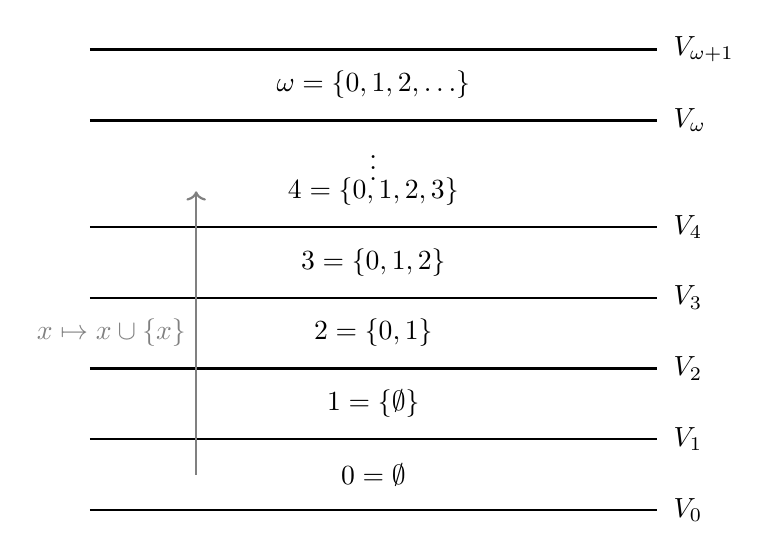
\begin{tikzpicture}[scale=0.9]
% V_alpha levels (rungs)
\foreach \name/\h in {V_0/0, V_1/1, V_2/2, V_3/3, V_4/4, V_\omega/5.5, V_{\omega+1}/6.5} {
  \draw[thick] (-4, \h) -- (4, \h);
  \node[anchor=west] at (4.1, \h) {$\name$};
}

% Mid-rung labels: each number lives in V_{n+1}, so we place it midway
% between V_n and V_{n+1}.
\node at (0, 0.5) {$0 = \emptyset$};
\node at (0, 1.5) {$1 = \{\emptyset\}$};
\node at (0, 2.5) {$2 = \{0,1\}$};
\node at (0, 3.5) {$3 = \{0,1,2\}$};
\node at (0, 4.5) {$4 = \{0,1,2,3\}$};
\node at (0, 4.95) {$\vdots$};
\node at (0, 6.0) {$\omega = \{0,1,2,\ldots\}$};

% Vertical guide for the "successor builds upward" intuition
\draw[->, thick, gray] (-2.5, 0.5) -- (-2.5, 4.5)
   node[midway, left, gray] {$x \mapsto x \cup \{x\}$};
\end{tikzpicture}
\caption{The cumulative hierarchy $V_\alpha$. Each natural number $n$ first
appears at level $V_{n+1}$. The set $\omega$ first appears at level
$V_{\omega+1}$.}
\label{fig:hierarchy}
\end{figure}

\section{A Representation Theorem}
\label{sec:representation}

We extract from the foregoing the following algebraic statement, which
expresses the structural fact that all encodings of the natural numbers
are mutually isomorphic.

\begin{definition}[Successor structure]\label{def:succ-struct}
A \emph{successor structure} is a triple $(X, x_0, s)$ where $X$ is a set,
$x_0 \in X$, and $s: X \to X$. A morphism $(X, x_0, s) \to (Y, y_0, t)$
is a function $f: X \to Y$ with $f(x_0) = y_0$ and $f \circ s = t \circ f$.
\end{definition}

\begin{definition}[Initial Peano structure]\label{def:init-peano}
A successor structure $(N, 0, S)$ is \emph{initial} (or a \emph{Peano
structure}) when, for every successor structure $(X, x_0, s)$, there exists
a unique morphism $h: (N, 0, S) \to (X, x_0, s)$.
\end{definition}

\begin{theorem}[Initiality of $\omega$]\label{thm:initiality}
$(\omega, 0_{\mathrm{vN}}, (\cdot)^+)$ is an initial Peano structure.
Equivalently: for every set $X$, every $a \in X$, and every $g: X \to X$,
there is a unique $f: \omega \to X$ with $f(0) = a$ and $f(n^+) = g(f(n))$.
This $f$ is the recursion theorem (\Cref{thm:recursion}).
\end{theorem}

\begin{proof}
This is precisely the recursion theorem, recast as initiality. Existence is
by recursion on $\omega$; uniqueness is by induction.
\end{proof}

\begin{theorem}[Uniqueness of Peano structures]\label{thm:uniqueness}
If $(N, 0, S)$ and $(N', 0', S')$ are both initial Peano structures, then
there is a unique isomorphism between them.
\end{theorem}

\begin{proof}
Universal property: by initiality of $(N, 0, S)$, there is a unique
$h: N \to N'$. By initiality of $(N', 0', S')$, there is a unique
$h': N' \to N$. The composites $h' \circ h$ and $h \circ h'$ are
endomorphisms of an initial structure, hence equal to the identity by
uniqueness.
\end{proof}

\begin{corollary}\label{cor:vN-Z-iso}
The von Neumann and Zermelo successor structures are isomorphic via a unique
isomorphism, namely $\Phi$ of \Cref{thm:peano-iso}.
\end{corollary}

This is the structural content that survives Benacerraf's critique. Both
encodings are initial Peano structures; they are therefore canonically
identified at the structural level. What differs is the
encoding-specific data: cardinalities of the carrier sets at each level,
membership relations, etc. The structural mathematics survives; the
junk does not.

\section{Bridge to Structuralism}
\label{sec:bridge}

\subsection{Reading the structuralist response}

The standard structuralist response to Benacerraf is to assert that
``numbers are positions in structures, not particular objects.'' Within
the set-theoretic perspective alone, this assertion is hard to formalize:
the structuralist seems to be invoking abstract structures that are not
themselves sets.

What Paper 03 will show is that the universal property of an initial
Peano structure is precisely the structuralist content the response was
gesturing at. \Cref{thm:initiality,thm:uniqueness} together say:

\begin{quote}
There is a structure (the initial successor structure), unique up to unique
isomorphism, defined entirely by its relationships with all other successor
structures. This structure can be \emph{implemented} in many ways inside
ZFC; no implementation is canonical, but every implementation is
equivalent to every other in the only way that matters --- via the
universal mapping property.
\end{quote}

\subsection{The set-theoretic perspective relocated}

We can therefore retract the temptation to read the von Neumann encoding
as ontology. The set-theoretic perspective is best understood as
\emph{realizing} or \emph{instantiating} a structural specification, not
as defining what the natural numbers \emph{are}. The number $58$ is not
the set $\{0,1,\ldots,57\}$; rather, the set $\{0,1,\ldots,57\}$ is one
particular ZFC-implementation of the position $58$ inside the abstract
initial successor structure.

\subsection{What set theory still gets right}

Despite Benacerraf's critique, the set-theoretic perspective is not
worthless. It contributes:

\begin{itemize}
\item \textbf{Existence.} Without an existence proof, the universal property
of \Cref{def:init-peano} is mere stipulation. Set theory shows that an
initial Peano structure exists (the axiom of infinity gives one), so the
specification is not vacuous.

\item \textbf{A working metatheory.} ZFC is rich enough to prove the
recursion theorem, define addition and multiplication, prove the soundness
of induction, and develop most of ordinary mathematics. The structural
specification needs a host theory; ZFC is one (other choices: ETCS, IZF,
HoTT itself).

\item \textbf{Cumulative hierarchy as a model of well-foundedness.} The
$V_\alpha$ stratification, while encoding-relative in detail, captures the
genuine structural fact that any well-founded iteration of \emph{some}
generative operation eventually exhausts what can be reached.

\item \textbf{Decidable arithmetic.} The recursive definitions of $+$,
$\cdot$, and $<$ are decidable; the resulting theory of arithmetic is
$\Sigma_1$-complete and useful in practice.
\end{itemize}

\subsection{What set theory misses}

\begin{itemize}
\item \textbf{Structural identity.} Set-theoretic equality is extensional:
two sets are equal iff they have the same elements. There is no native
notion of ``equal as Peano structures'' inside ZFC; isomorphism must be
defined externally and tracked manually.

\item \textbf{Encoding-independence.} As shown, the set-theoretic statement
``$2 \in 3$'' is encoding-relative. The structural statement ``$\mathrm{succ}(\mathrm{succ}(0)) < \mathrm{succ}^3(0)$'' is not.

\item \textbf{Universal properties as theorems, not metatheorems.} In
ZFC, ``$\omega$ is initial'' is a theorem, but the very statement of
initiality requires quantifying over class-many successor structures
(properly handled, but unwieldy). In a categorical or type-theoretic
foundation, the universal property is the \emph{definition} and the
existence/uniqueness are immediate consequences.

\item \textbf{Univalence.} ZFC has no analog of the univalence axiom of
HoTT; it cannot internalize ``isomorphic structures are the same'' as a
theorem of the system. The closest one comes is to work systematically
``up to isomorphism,'' which is a metatheoretic discipline rather than
a feature of the formalism.
\end{itemize}

\subsection{Forward to Paper 03}

The next paper in the series develops the universal-property level
explicitly: a Natural Number Object in any category with a terminal object,
the categorical NNO, the relationship between NNO and induction, and the
extraction of arithmetic operations from initiality alone. The bridge from
this paper to the next is precisely the move from
\Cref{thm:initiality}'s ``$\omega$ is initial in $\mathbf{Set}^{\bullet,\to}$''
to the encoding-free formulation
``$N$ is initial in any category $\mathcal{C}^{\bullet,\to}$ with a terminal
object.''

\section{Haskell Implementation}
\label{sec:haskell}

The accompanying Haskell code (\texttt{src/02-set-theoretic/}) implements
both encodings, defines a common Peano interface they both satisfy, and
provides a converter realizing the canonical isomorphism $\Phi$ of
\Cref{thm:peano-iso}.

\subsection{The hereditarily finite set type}

We model pure sets as a recursive datatype:

\begin{lstlisting}
-- A finite set built recursively from the empty set.
-- Extensional equality is enforced in the Eq instance by sorting
-- and deduplicating the underlying list before comparison; a
-- canonical-form helper (omitted here) makes this efficient.
newtype HFSet = HFSet { elements :: [HFSet] }
  deriving (Show)

instance Ord HFSet where
  compare (HFSet xs) (HFSet ys) =
    compare (sort xs) (sort ys)

instance Eq HFSet where
  HFSet xs == HFSet ys = sort xs == sort ys

emptySet :: HFSet
emptySet = HFSet []
\end{lstlisting}

\subsection{Von Neumann encoding}

\begin{lstlisting}
-- Successor: x |-> x \cup {x}
vnSucc :: HFSet -> HFSet
vnSucc x = HFSet (elements x ++ [x])

vnEncode :: Int -> HFSet
vnEncode 0 = emptySet
vnEncode n = vnSucc (vnEncode (n - 1))
\end{lstlisting}

\subsection{Zermelo encoding}

\begin{lstlisting}
-- Successor: x |-> {x}
zSucc :: HFSet -> HFSet
zSucc x = HFSet [x]

zEncode :: Int -> HFSet
zEncode 0 = emptySet
zEncode n = zSucc (zEncode (n - 1))
\end{lstlisting}

\subsection{The Peano interface}

A typeclass captures the structural specification independent of either
encoding:

\begin{lstlisting}
class Peano a where
  zero :: a
  suc  :: a -> a
  isZero :: a -> Bool
  pred_ :: a -> Maybe a   -- partial; (-) on naturals is partial

instance Peano HFSet where
  -- These instances need to be coupled with a tagged type to
  -- disambiguate vN vs Zermelo; see VNNat and ZNat in the source.
\end{lstlisting}

The full source disambiguates by tagging: \texttt{newtype VNNat = VNNat HFSet}
and \texttt{newtype ZNat = ZNat HFSet}, each with its own \texttt{Peano} instance.
The main demonstration in \texttt{Main.hs} computes both encodings of
$0,1,\ldots,5$, prints them, verifies the Peano axioms by construction (e.g.\
$\mathrm{succ}(m) = \mathrm{succ}(n) \implies m = n$ via injectivity of the
constructor), and applies the canonical isomorphism to convert between them.

\subsection{Junk theorems made explicit}

The Haskell code also includes a function that demonstrates a junk theorem
empirically:

\begin{lstlisting}
-- Demonstrate that "1 in 3" depends on encoding.
junkTheorem :: IO ()
junkTheorem = do
  let one_vN  = vnEncode 1; three_vN = vnEncode 3
  let one_Z   = zEncode  1; three_Z  = zEncode  3
  putStrLn $ "vN: 1 in 3 = " ++ show (one_vN `inVN` three_vN)
  putStrLn $ "Z:  1 in 3 = " ++ show (one_Z  `inZ`  three_Z)
  -- Output:
  --   vN: 1 in 3 = True   (since 3_vN = {0,1,2})
  --   Z:  1 in 3 = False  (since 3_Z  = {2}; only 2 is in it)
\end{lstlisting}

This program is a working witness that the encoding is genuinely choosing
between distinct sets, not merely between distinct notations.

\section{Discussion}
\label{sec:discussion}

\subsection{Comparison with logicism and constructivism}

The set-theoretic foundationalism we have presented is closer to
Russell--Whitehead's logicist program than to a strict constructivism.
The naturals are obtained by an unbounded inductive process whose existence
is asserted by an axiom (Infinity). This is not predicatively justified
in a strict sense (the inductive set is defined as the intersection of
\emph{all} inductive sets, a quantification over a complete totality), but
it is mainstream classical mathematics.

Constructive alternatives --- IZF, CZF, Martin-L\"of type theory --- avoid
this by treating $\mathbb{N}$ as primitive (an inductive type) rather than
as a derived set. Paper 05 treats this perspective via HoTT.

\subsection{Comparison with categorical foundations}

Lawvere's Elementary Theory of the Category of Sets (ETCS,
\cite{lawvere1964}) gives a categorical axiomatization of the category
$\mathbf{Set}$ that is bi-interpretable with bounded Zermelo set theory
plus replacement (McLarty \cite{mclarty2004}). In ETCS, the natural number
object is specified by its universal property (Paper 03's level), not by a
particular encoding. ETCS is therefore structurally cleaner than ZFC for
foundational purposes, while equally adequate for ordinary mathematics. The
underlying functorial-semantics machinery is developed in Lawvere
\cite{lawvere1963}, and the broader topos-theoretic context is treated by
Mac Lane and Moerdijk \cite{maclane-moerdijk}.

\subsection{Limitations of this paper}

We have not discussed:
\begin{itemize}
\item \emph{Large cardinal hypotheses.} Inaccessible, measurable, etc.
cardinals refine the cumulative hierarchy beyond the ordinals reachable
in vanilla ZFC. They are foundational for set theory but tangential to
the natural-numbers question.

\item \emph{The constructible universe $L$.} G\"odel's inner model
exhibits a minimal model of ZFC; the natural numbers are the same in $L$
as in $V$, so this is not pertinent.

\item \emph{Forcing.} Independence results do not affect our development.

\item \emph{Alternative set theories.} NF (Quine), KP (Kripke--Platek),
and other systems give variant encodings; we have considered only ZFC.
\end{itemize}

\subsection{What this paper has accomplished}

We have presented two distinct set-theoretic encodings of the natural
numbers (von Neumann ordinals and Zermelo nested singletons), shown that
both satisfy the Peano axioms, and identified the encoding-relative facts
(``junk theorems'') that distinguish them. We have located the natural
numbers in the cumulative hierarchy and proven a representation theorem
identifying all initial Peano structures up to unique isomorphism. We have
described the structuralist response (numbers are positions, not sets)
and pointed forward to the universal-property and HoTT formulations of
that response.

\section{Conclusion}
\label{sec:conclusion}

The set-theoretic perspective gives us $\omega$ via the axiom of infinity
and the recursive successor $x \mapsto x \cup \{x\}$. It supports a full
arithmetic, fits cleanly into the cumulative hierarchy, and makes the
natural numbers concrete: the number $58$ \emph{is} the set $\{0,1,\ldots,57\}$
--- in the von Neumann encoding.

But the qualifier ``in the von Neumann encoding'' is fatal to the
foundationalist ambition. Zermelo's encoding is equally valid; so is the
Peano-axiomatic specification with no encoding at all; and so are the
many other encodings one could devise. Each gives a working arithmetic
that satisfies the Peano axioms, but each disagrees with the others on
internal questions about element-of, cardinality, and rank. These
disagreements are not pathologies; they are evidence that no encoding
gives \emph{the} natural numbers --- only one realization of them.

What we have learned is that the natural numbers are characterized
structurally, not extensionally. This characterization is the universal
property of an initial Peano structure (\Cref{def:init-peano}), and its
sharpening into the categorical Natural Number Object will occupy
Paper 03. The set-theoretic perspective remains useful as a metatheory
and an existence proof, but the identity of the natural numbers
themselves lives at one level of abstraction higher.

\subsection*{Acknowledgments}

This paper is part of the YonedaAI Univalent Correspondence series. The
series approaches a single mathematical object --- the natural numbers ---
through six distinct lenses, and shows in the synthesis volume that under
the univalence axiom, all six perspectives become literally the same
mathematical content rather than analogous content. We thank the
anonymous referees of the series for sharpening many arguments.

\begin{thebibliography}{99}

\bibitem{benacerraf1965}
P.~Benacerraf, ``What Numbers Could Not Be,''
\emph{The Philosophical Review}, vol. 74, no. 1, pp. 47--73, 1965.

\bibitem{benacerraf1973}
P.~Benacerraf, ``Mathematical Truth,''
\emph{The Journal of Philosophy}, vol. 70, no. 19, pp. 661--679, 1973.

\bibitem{frege1884}
G.~Frege, \emph{Die Grundlagen der Arithmetik},
W. Koebner, Breslau, 1884.

\bibitem{halmos1960}
P.~Halmos, \emph{Naive Set Theory},
Van Nostrand, 1960.

\bibitem{kunen1980}
K.~Kunen, \emph{Set Theory: An Introduction to Independence Proofs},
North-Holland, 1980.

\bibitem{lawvere1964}
F. W.~Lawvere, ``An Elementary Theory of the Category of Sets,''
\emph{Proc. Nat. Acad. Sci. USA}, vol. 52, pp. 1506--1511, 1964.

\bibitem{lawvere1963}
F. W.~Lawvere, ``Functorial Semantics of Algebraic Theories,''
PhD thesis, Columbia University, 1963.

\bibitem{maclane-moerdijk}
S.~Mac Lane and I.~Moerdijk, \emph{Sheaves in Geometry and Logic},
Springer, 1992.

\bibitem{mclarty2004}
C.~McLarty, ``Exploring Categorical Structuralism,''
\emph{Philosophia Mathematica}, vol. 12, no. 1, pp. 37--53, 2004.

\bibitem{principia}
A. N.~Whitehead and B.~Russell, \emph{Principia Mathematica}, Cambridge
University Press, 1910--1913.

\bibitem{shoenfield1967}
J. R.~Shoenfield, \emph{Mathematical Logic},
Addison-Wesley, 1967.

\bibitem{shapiro1997}
S.~Shapiro, \emph{Philosophy of Mathematics: Structure and Ontology},
Oxford University Press, 1997.

\bibitem{suppes1960}
P.~Suppes, \emph{Axiomatic Set Theory},
Van Nostrand, 1960.

\bibitem{vonNeumann1923}
J.~von Neumann, ``Zur Einf\"uhrung der transfiniten Zahlen,''
\emph{Acta litt. ac scient. Reg. Univ. Hung. Francisco-Josephinae},
sectio sci. math., vol. 1, pp. 199--208, 1923.

\bibitem{HoTTBook}
The Univalent Foundations Program, \emph{Homotopy Type Theory: Univalent
Foundations of Mathematics}, Institute for Advanced Study, 2013.
\href{https://homotopytypetheory.org/book}{homotopytypetheory.org/book}.
arXiv:1308.0729.

\bibitem{zermelo1908}
E.~Zermelo, ``Untersuchungen \"uber die Grundlagen der Mengenlehre I,''
\emph{Math. Ann.}, vol. 65, pp. 261--281, 1908.

\end{thebibliography}

\end{document}
